\documentclass{article}
\usepackage{graphicx} % Required for inserting images
\usepackage{xcolor}

\usepackage[draft,inline,nomargin]{fixme}
\fxsetup{theme=color}
\definecolor{jacolor}{RGB}{200,40,0}
\FXRegisterAuthor{ja}{aja}{\color{jacolor}JA}
\definecolor{accolor}{HTML}{008080}
\FXRegisterAuthor{ac}{anac}{\color{accolor}AC}
\definecolor{cpcolor}{RGB}{0,200,40}
\FXRegisterAuthor{cp}{ancp}{\color{cpcolor}CP}

\newcommand{\GIOC}{\texttt{GIOC}}

\title{Librerias \GIOC}
\author{Amado A. Cabrera}
\date{July 2025}

\begin{document}

\maketitle

\section{Paquetes que componen \GIOC}
El paquete \GIOC{} \acnote{esa es mi propuesta para el nombre de la libreria más grande} está compuesto de varias sub-librerias \acnote{también esa es mi propuesta}:
\begin{enumerate}
    \item \texttt{Meta}:\\
    Librería con todas las herramientas para crear paquetes o  tareas relacionadas más con el formato o estructura de notebooks que con código diario (e.g. \texttt{OffSpellErrors}, \texttt{OnSpellErrors} o las cosas para paquetes de \texttt{ForScience}, entre otras).

    \item \texttt{General}:\\
    Librería con herramientas variadas que se usan en el código, pero que no están relacionadas con la física (e.g. \texttt{Lg}, \texttt{APITeX}, \texttt{My5PointStar}, entre otras).

    \item \texttt{Quantum}:\\
    Librería con funciones de mecánica cuántica que apliquen a variedad de modelos (e.g. \texttt{MatrixPartialTrace}, \texttt{ApplyOperator}, \texttt{RandomQubitState}, entre otras).

    \item Libreria por modelo:\\
    Cada modelo en el que se trabaje puede tener su propio modulo con funciones específicas para ese modelo, ``estructuras de datos'' propias, graficas, etc. La estructura de cada sub-paquete se organizará en subcarpetas y archivos por cada función nueva \acnote{o no, solo es mi sugerencia xdddd} (e.g. \texttt{QW\textasciigrave NewDTQW}).

    \item \texttt{Experimental}:\\
    En esta librería creo que se pueden construir funciones que se quieran \textit{testear} extensivamente o para desarrollar paquetes. La idea sería que el contexto experimental no cargue por defecto o se tenga que llamar con el nombre del contexto para cada función.

    \item \texttt{Deprecated}:\\
    Si se quiere mantener ciertas funciones obsoletas (porque hay unas mejores que esas), pero se necesita mantenerlas para poder replicar ciertos resultados sin reescribir toda la lógica del código se pueden mantener aquí. El contexto se trataría igual que el del paquete \texttt{Experimental}, no cargarlo por defecto o llamarlos con nombre completo (e.g. \texttt{QW\textasciigrave NumericDTQW}).
\end{enumerate}

\section{Convenio de sintaxis}

\begin{enumerate}
\item Usar de las funciones de \texttt{ForScience} para formatear bonito los mensajes
de uso 
\item Nombres de funciones claros y explícitos según lo que hagan
\item Mensajes de uso en la forma estándar de Mathematica, siendo claros con 
los argumentos de las funciones y qué retorna
\item Breaks obligatorios antes de las 80 columnas
\item Si la función tiene opciones. Colocar al final de la definición de la primer
definición de uso (capaz tiene más de una definición las opciones disponibles
\end{enumerate}

\begin{figure}[hbt]
\centering
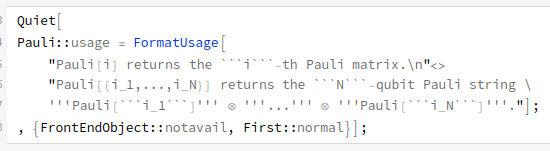
\includegraphics[width=\textwidth]{estandar1.png}
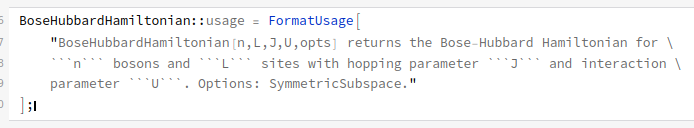
\includegraphics[width=\textwidth]{estandar2.png}
\end{figure}

\end{document}
